% Source for Figure 2 in the review paper.
% Compile standalone with pdflatex if a regenerated figure is required.
\documentclass[tikz,border=6pt]{standalone}
\usepackage{tikz}
\usetikzlibrary{arrows.meta}
\begin{document}
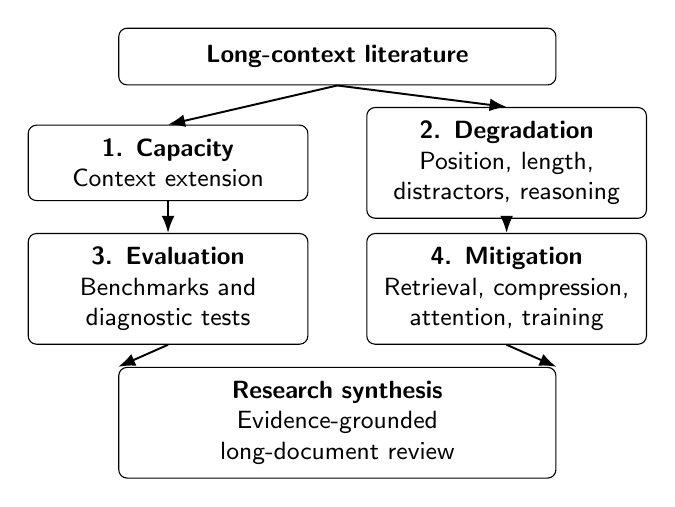
\begin{tikzpicture}[
  font=\sffamily\small,
  box/.style={draw, rounded corners=3pt, align=center, minimum height=0.72cm, inner sep=5pt, text width=3.2cm},
  root/.style={draw, rounded corners=3pt, align=center, minimum height=0.72cm, inner sep=5pt, text width=5.2cm},
  bottom/.style={draw, rounded corners=3pt, align=center, minimum height=0.72cm, inner sep=5pt, text width=5.2cm},
  arrow/.style={-Latex, line width=0.7pt}
]
\node[root] (root) at (0,0) {\textbf{Long-context literature}};
\node[box] (cap) at (-2.15,-1.35) {\textbf{1. Capacity}\\Context extension};
\node[box] (deg) at (2.15,-1.35) {\textbf{2. Degradation}\\Position, length, distractors, reasoning};
\node[box] (eval) at (-2.15,-2.95) {\textbf{3. Evaluation}\\Benchmarks and diagnostic tests};
\node[box] (mit) at (2.15,-2.95) {\textbf{4. Mitigation}\\Retrieval, compression, attention, training};
\node[bottom] (synth) at (0,-4.65) {\textbf{Research synthesis}\\Evidence-grounded long-document review};
\draw[arrow] (root.south) -- (cap.north);
\draw[arrow] (root.south) -- (deg.north);
\draw[arrow] (cap.south) -- (eval.north);
\draw[arrow] (deg.south) -- (mit.north);
\draw[arrow] (eval.south) -- (synth.north west);
\draw[arrow] (mit.south) -- (synth.north east);
\end{tikzpicture}
\end{document}
